% =====================================================================
%  From Replayable Traces to Provenance-Aware Rule Fusion
%  Bounded auditability claims for reinforcement learning agents
%
%  Compile:  pdflatex DeepSeek -> bibtex DeepSeek -> pdflatex DeepSeek x2
%  Requires: references.bib (same directory). No external figure files.
% =====================================================================
\documentclass[11pt,a4paper]{article}

\usepackage[margin=1in]{geometry}
\usepackage{amsmath,amssymb,amsthm}
\usepackage{booktabs}
\usepackage{array}
\usepackage{tabularx}
\usepackage{graphicx}
\usepackage{tikz}
\usetikzlibrary{positioning,arrows.meta,shapes.geometric,calc}
\usepackage{float}
\usepackage{algorithm}
\usepackage{algpseudocode}
\usepackage{xcolor}
\usepackage{enumitem}
\usepackage{microtype}
\usepackage[round]{natbib}
\usepackage[font=small,labelfont=bf]{caption}
\usepackage[hidelinks]{hyperref}

\newtheorem{definition}{Definition}
\newtheorem{proposition}{Proposition}
\newtheorem{remark}{Remark}

\setlist[itemize]{leftmargin=1.4em,topsep=2pt,itemsep=1pt,parsep=0pt}
\setlist[enumerate]{leftmargin=1.6em,topsep=2pt,itemsep=1pt,parsep=0pt}

% Shorthand used only in figure and table code.
\newcommand{\tick}{\textcolor{black!70}{\rule{0.6pt}{2.6ex}}}

\title{\vspace{-1.2em}From Replayable Traces to Provenance-Aware Rule Fusion:\\ Bounded Auditability Claims for Reinforcement Learning Agents\vspace{-0.4em}}
\author{Anonymous Author(s)}
\date{\today}

\begin{document}
\maketitle

\begin{abstract}
\noindent
Reinforcement learning (RL) agents are increasingly asked to justify their decisions, yet the word \emph{auditability} bundles at least six different questions: whether a recorded execution is intact and replayable; whether a trace can be recoded without loss; whether induced rules cover held-out states; whether two agents that share symbolic rules actually behave alike; whether rules can be composed with visible provenance; and whether a value model is reliable enough to compose policies at all. Passing one test does not imply passing another, and a single score conceals the difference. We report a bounded study that measures each question separately. Eight agents per task, trained for 300 episodes on CartPole-v1 and Acrobot-v1, share one frozen state symbolizer; a separate six-seed designed coordination task lets us manipulate a learned symbol directly. Our first result is negative and load-bearing: exact state--action rule overlap across CartPole seeds is substantial (mean pairwise Jaccard $0.5572$), yet the two agents agree on only $51.36\%$ of actions (95\% episode-cluster bootstrap interval $[50.48,52.26]$) when both are applied to $10{,}000$ fresh held-out raw states. Symbolic overlap does not license a behavioural-consensus claim. A provenance-aware fusion layer records the candidate rules, their source banks, the arbitration outcome and any fallback for every decision, and emits a hash-linked trace that an independent verifier resolves and replays. On Acrobot the fused policy scores $-443.37$ against $-500.00$ for the best single actor, but $89.24\%$ of its decisions are conflicts, and ablating the arbiter shows random selection among available source rules beating every deterministic variant tested, including the deployed one --- an anomaly we report as unexplained rather than as a method. In the designed task, matched-support interventions on the information-bearing symbol shift receiver action probability by $0.998366$ on average across six seeds. A fitted-Q comparator fails its own pre-declared quality checks and is reported as a non-claim. We claim bounded existence, not general auditability.
\end{abstract}

% =====================================================================
\section{Introduction}
\label{sec:intro}

\subsection{A concrete situation}

An engineer is handed a log of an agent's decisions and asked to justify one of them. Three reflexes suggest themselves. First, replay the log: re-execute the recorded actions in the recorded environment and check that every transition reproduces. Second, induce rules from the log and show which rule fired at the decision in question. Third, if several agents are involved, show which agent supplied the rule that was used. Each reflex is reasonable, and each answers a different question. Replay tells us the record is faithful. An induced rule tells us that some regularity was observed. Attribution tells us where a rule came from. None of the three establishes that the rule \emph{governed} the decision, and none of them tells us what to do when two agents' rules disagree.

This paper is about keeping those questions apart. We deliberately refuse to aggregate them into an ``auditability score'', because the evidence we present shows that the questions can come apart sharply: in our largest experiment, two agents whose rule sets overlap by more than half agree on barely more than half of their actions on fresh states. Figure~\ref{fig:questions} names the six questions we distinguish and states, for each, what it does not on its own license.

\begin{figure}[t]
\centering
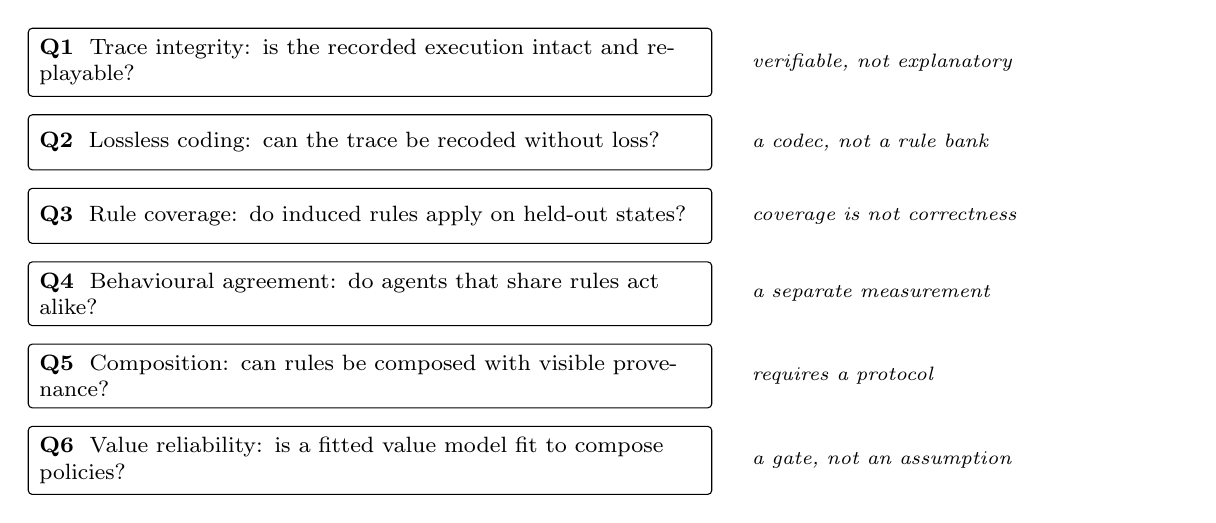
\begin{tikzpicture}[font=\footnotesize, node distance=2.2mm,
  q/.style={draw, rounded corners=1.5pt, align=left, inner sep=4pt, text width=84mm, minimum height=7mm},
  tag/.style={font=\scriptsize\itshape, align=left, text width=54mm}]
\node[q] (q1) {\textbf{Q1}\ \ Trace integrity: is the recorded execution intact and replayable?};
\node[q, below=of q1] (q2) {\textbf{Q2}\ \ Lossless coding: can the trace be recoded without loss?};
\node[q, below=of q2] (q3) {\textbf{Q3}\ \ Rule coverage: do induced rules apply on held-out states?};
\node[q, below=of q3] (q4) {\textbf{Q4}\ \ Behavioural agreement: do agents that share rules act alike?};
\node[q, below=of q4] (q5) {\textbf{Q5}\ \ Composition: can rules be composed with visible provenance?};
\node[q, below=of q5] (q6) {\textbf{Q6}\ \ Value reliability: is a fitted value model fit to compose policies?};
\node[tag, right=4mm of q1] (t1) {verifiable, not explanatory};
\node[tag, right=4mm of q2] (t2) {a codec, not a rule bank};
\node[tag, right=4mm of q3] (t3) {coverage is not correctness};
\node[tag, right=4mm of q4] (t4) {a separate measurement};
\node[tag, right=4mm of q5] (t5) {requires a protocol};
\node[tag, right=4mm of q6] (t6) {a gate, not an assumption};
\end{tikzpicture}
\caption{Six questions that the word \emph{auditability} commonly bundles into a single score. They are independent predicates, and the evidence below shows they can point in opposite directions: in our largest experiment the record is maximally intact (Q1) while the rule-based account of behaviour is at chance (Q4). The right-hand column states what each question, taken alone, does not license.}
\label{fig:questions}
\end{figure}

\subsection{Three limitations of existing approaches}
\label{sec:intro-limits}

\paragraph{Limitation 1: interpretability work is artifact-centric, not execution-centric.}
A substantial literature produces interpretable artifacts: policies expressed in readable program languages that admit symbolic verification \citep{verma2018}, and models that are interpretable by construction rather than explained after the fact \citep{rudin2019,lipton2018}. These artifacts can be inspected. But an inspectable artifact is not a faithful record of what a particular execution did, and the literature that argues for interpretable-by-design models is explicitly a critique of post-hoc explanation, not a specification of what a tamper-evident execution record must contain.

\paragraph{Limitation 2: value-based policy composition is opaque in exactly the place provenance is needed.}
Successor features and generalised policy improvement compose policies through value functions and can improve performance without additional learning \citep{barreto2017,thakoor2022}. The composition, however, is a maximum over estimated values. It does not expose which source policy produced a given decision, it has no notion of a state where \emph{no} source has support, and its correctness depends on the fitted value model being good enough --- a condition that off-policy evaluation studies show is frequently violated \citep{voloshin2021,le2019}.

\paragraph{Limitation 3: measurement caution is not a provenance protocol.}
Work on emergent communication establishes that intuitive metrics such as message--action correlation can mislead, and argues for interventional tests \citep{lowe2019,kharitonov2019,chaabouni2020}. Reproducibility work establishes that nondeterminism must be controlled and documented before an execution can be replayed \citep{nagarajan2018}. Both give us reasons to distrust measurements. Neither supplies a mechanism for recording, resolving, and rejecting provenance claims about individual decisions.

\subsection{Problem and objective}
\label{sec:intro-problem}

We ask what a replayable trajectory, plus a set of rules induced from it, can actually support. Our objective is to build the smallest mechanism that makes rule-level composition \emph{provenance-visible and independently checkable}, and then to find out, by experiment, which claims that mechanism does and does not license. The second half of that objective matters as much as the first: the contribution of this paper is as much a set of explicit counterexamples as it is a system.

\subsection{Challenges: why direct reuse fails}
\label{sec:intro-challenges}

\paragraph{Challenge 1: compression is not explanation.}
A grammar induced from a sequence can reconstruct that sequence exactly and still say nothing about which rule governed any decision. Sequence-grammar induction is a compression method; its own authors caution that the rules it produces are not automatically a generalised grammar \citep{nevillmanning1997}. Conflating a lossless codec with a policy explanation is the first failure we had to undo.

\paragraph{Challenge 2: symbolic overlap is not behavioural consensus.}
Overlap between two induced rule sets is a statistic about syntax. Whether the two agents that produced those rule sets choose the same action on the same state is a separate measurement, and the two need not agree.

\paragraph{Challenge 3: trace integrity is not training-process audit.}
Re-executing recorded transitions verifies the record. It does not recover policy weights over time, optimizer state, gradients, or the random-number state that produced them, and it cannot establish that the recorder was honest.

\paragraph{Challenge 4: provenance needs a protocol, not a data structure.}
Storing a source identifier next to a decision is trivial. Making that identifier \emph{checkable} requires deciding who may write which field, when a decision becomes immutable, what a verifier is entitled to reject, and how the answer changes when a rule bank is revised. Those are protocol questions, and we answer them with an explicit state machine rather than with a schema.

\subsection{Method components mapped to challenges}
\label{sec:intro-mapping}

The four challenges drive four design decisions, each of which is a separate component in Section~\ref{sec:method}.
\begin{itemize}
  \item \textbf{C1 $\rightarrow$ separation of codec and rule bank.} We maintain two distinct symbolic objects: a lossless sequence grammar over the recorded trace, whose quality we report as a two-part code length, and a state--action rule bank, whose quality we report as coverage and action agreement. Neither is used as evidence for the other.
  \item \textbf{C2 $\rightarrow$ an independent behavioural estimand.} Overlap is reported alongside an experiment that applies two frozen actors to the same fresh held-out raw states and measures action agreement with an episode-cluster balanced estimator.
  \item \textbf{C3 $\rightarrow$ an explicitly scoped audit instrument.} The instrument records per-step rows, an optimizer-update ledger, calibration metadata and rule-provenance snapshots, links them into a hash chain, and replays logged transitions. Its scope statement lists what it cannot identify.
  \item \textbf{C4 $\rightarrow$ a decision protocol with role-separated authority.} A finite-state protocol fixes who writes the decision, who seals it, who verifies it, and what each party is entitled to reject.
\end{itemize}

\subsection{Contributions}
\label{sec:intro-contrib}

\begin{enumerate}
  \item \textbf{Provenance-aware rule fusion with explicit decision classes.} A fusion layer that classifies every decision as agreement, single-source, conflict, or blind spot; that records the candidate rules, their source banks and their arbitration outcome; and that emits a hash-linked trace resolvable against those sources. (Primary; claim budget \textbf{CB1}.)
  \item \textbf{A negative result that constrains the whole programme.} On $10{,}000$ fresh held-out CartPole states, two agents with exact rule Jaccard $0.5833$ agree on $51.36\%$ of actions. Rule-set overlap does not support a shared-policy-core claim. (Primary; \textbf{CB2}.)
  \item \textbf{Composition results with their decision mix reported.} Fused mean returns of $205.96$ (CartPole) and $-443.37$ (Acrobot) against best single actors of $163.65$ and $-500.00$, together with coverage, conflict and blind-spot rates that determine how the means should be read. (Secondary; \textbf{CB3}.)
  \item \textbf{An arbitration sensitivity study, including an unexplained anomaly.} Nine matched-seed arbiter variants plus a random-selection control; random selection among available source rules beats every deterministic variant tested. (Secondary/diagnostic; \textbf{CB4}.)
  \item \textbf{A causal test of a learned symbol in a designed task.} Matched-support interventions on the information-bearing symbol position shift receiver action probability by $0.998366$ on average across six seeds. (Secondary; \textbf{CB5}.)
  \item \textbf{A trace-audit instrument with a stated scope.} Hash-chain, ledger, provenance-resolution and environment-replay checks over $1{,}725{,}655$ and $2{,}544{,}513$ recorded rows. (Instrument; \textbf{CB6}.)
\end{enumerate}

The remainder of the paper is organised as follows. Section~\ref{sec:related} positions the work. Section~\ref{sec:setting} fixes notation and estimands. Section~\ref{sec:history} is a failure-driven design history, which is where the argument is actually made. Section~\ref{sec:method} formalises what survived. Sections~\ref{sec:setup} and~\ref{sec:results} report the experiments. Section~\ref{sec:discussion} discusses, Section~\ref{sec:limits} states limitations, and Section~\ref{sec:conclusion} concludes.

% =====================================================================
\section{Related Work}
\label{sec:related}

\subsection{Axis 1: research direction}

\emph{Assumption.} Work on interpretable RL assumes that the obstacle to trust is the opacity of the policy representation, and that supplying a readable representation removes it.

\emph{Demonstrated achievement.} Programmatically interpretable RL learns policies in a readable language and verifies them symbolically \citep{verma2018}; interpretability research argues more broadly that models should be constrained to be interpretable rather than explained afterwards \citep{rudin2019,lipton2018}.

\emph{Conditions of failure.} The assumption fails when the question is not ``what policy was learned?'' but ``did this particular execution proceed as recorded, and which source produced this particular decision?''. A readable policy can be inspected without any guarantee that the execution record matches it. Interpretability is a property of an artifact; auditability is a property of a record and a protocol.

\emph{Relationship to the present work.} We treat readability as orthogonal. Our rule banks are readable in a weak sense (symbolic state conditions mapped to actions), but we never claim they explain decisions, and we measure separately whether they even predict them.

\subsection{Axis 2: methodology}

\emph{Rule-based.} Induced symbolic rules are inspectable and cheap to compose, but the induction step is a compression step and inherits its ambiguities \citep{nevillmanning1997}. Our Section~\ref{sec:history} documents what happened when we assumed otherwise.

\emph{Learned, value-based.} Successor features and geometric policy composition compose policies through value functions \citep{barreto2017,thakoor2022}. This is powerful and, unlike rule fusion, has a theoretical basis for improvement. Its dependence on value accuracy is a real constraint rather than a formality: comparative studies of off-policy evaluation report substantial and uneven error \citep{voloshin2021,le2019}, and we replicate that difficulty in Section~\ref{sec:res-gpi}.

\emph{Protocol-based.} Emergent-communication research supplies the closest methodological precedent: it distinguishes correlation from causal influence and prescribes interventions over observational metrics \citep{lowe2019,kharitonov2019}. Hash-linked, tamper-evident records are standard in the time-stamping literature \citep{haber1991} and are used here only as a mechanism, not as a contribution.

\emph{Why the transport distinction is not a methodological paradigm.} Our fusion layer is a deterministic kernel: it makes no new generation calls, and changing how its decisions are stored or transmitted would not change the scientific question. We therefore treat the decision protocol as an instrument and keep its description short (Section~\ref{sec:method-audit}), rather than presenting it as a method contribution.

\subsection{Axis 3: conflicting findings}

We did not find a verified body of literature that directly contradicts the specific measurements reported here, because the measurements are specific to our configuration. What the literature does contradict is the inference we were initially tempted to make: that symbolic overlap between two learned representations indicates shared behaviour. Work on emergent communication and compositionality warns against exactly this inference for messages \citep{lowe2019,chaabouni2020}, and we find it fails for induced state--action rules as well. We therefore do not claim a novel conflict; we claim an instance of a known warning in a setting where the warning is easy to ignore.

\paragraph{Bounded positioning.} Under the conditions we test --- two benchmark control tasks, one shared symbolizer per task, a fixed software and CPU configuration, and rule banks admitted at a fixed support and confidence --- a provenance-aware rule layer makes the composition of learned rules \emph{inspectable and replayable}, and on Acrobot it produces a policy whose mean return exceeds the best single source actor. We do not show that it beats value-based composition, which we could not validate here at all, nor that the advantage transfers to other tasks. Where value accuracy is reliable, value-based composition may remain preferable; where a decision must be attributable to a named source, a rule layer has an advantage our experiments do not establish for value methods.

% =====================================================================
\section{Problem Setting and Notation}
\label{sec:setting}

\subsection{Objects}

An environment is a partially observed control process with observation space $\mathcal{X}\subseteq\mathbb{R}^{d}$, action space $\mathcal{A}$, and transition kernel $T$ \citep{sutton2018}. A \emph{source policy} $\pi_{s}$ is a stochastic or deterministic map $\mathcal{X}\to\Delta(\mathcal{A})$ obtained by training. We train $S$ source policies per task, indexed by seed $s\in\{11,29,43,71,101,149,211,307\}$.

A \emph{trajectory} $\tau = (x_{0},a_{0},r_{0},\omega_{0},x_{1},\dots)$ records observations, actions, rewards and termination flags. A \emph{record} $c$ is a canonical serialisation of one trajectory row together with the metadata needed to replay it.

A \emph{state symbolizer} $\varphi$ maps raw observations to discrete symbols. A \emph{rule bank} $R_{s}$ maps symbolic states to at most one action. A \emph{fusion policy} $\pi_{f}$ composes the source policies through their rule banks and a fallback. A \emph{decision trace} is the sequence of records emitted by $\pi_{f}$.

\subsection{Quantities of interest and their units}

We keep the following quantities distinct throughout, because collapsing them is the error this paper is about.

\begin{itemize}
  \item \textbf{Rule overlap} $J_{s,s'}$: Jaccard similarity between the exact symbolic rule sets of seeds $s$ and $s'$. A set statistic, unit-free.
  \item \textbf{Behavioural agreement} $\bar{A}_{s,s'}$: the fraction of fresh held-out raw states on which two frozen actors select the same action. A behavioural measurement.
  \item \textbf{Rule coverage} $\gamma$: the fraction of decisions at which at least one rule bank applies.
  \item \textbf{Conflict rate} $\chi$: the fraction of decisions at which the banks disagree.
  \item \textbf{Blind-spot rate} $\beta$: the fraction of decisions at which no bank applies.
  \item \textbf{Return} $G(\pi)$: undiscounted episode return under a policy, reported as a mean over a fixed set of evaluation reset seeds, with the median reported alongside.
  \item \textbf{Paired difference} $\Delta$: the mean over evaluation episodes of the per-episode return difference between two policies evaluated on identical reset seeds.
  \item \textbf{Two-part code length} $W$: bits required to encode a trace under an induced grammar, reported as a diagnostic of the codec only.
\end{itemize}

\subsection{Falsifiable predictions}

We state predictions before reporting any result, so that they can be contradicted. Predictions \textbf{P1}--\textbf{P8} are listed in Table~\ref{tab:pred} in Section~\ref{sec:setup-pred}, immediately before the results, and each is given a status in Section~\ref{sec:results}.

% =====================================================================
\section{A Failure-Driven Design History}
\label{sec:history}

The mechanism in Section~\ref{sec:method} is the residue of six failed or partially failed attempts. We present them in order because the order is the argument: each repair was forced by a specific observation, and each repair left a specific residual boundary. Figure~\ref{fig:history} gives the sequence at a glance; the subsections that follow give the evidence for each stage.

\begin{figure}[t]
\centering
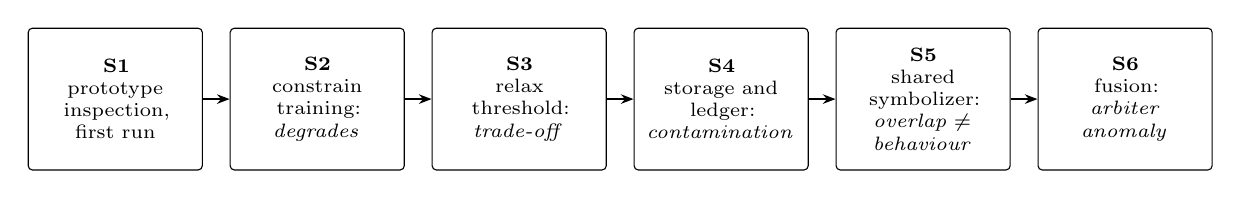
\begin{tikzpicture}[font=\scriptsize, node distance=3.4mm,
  b/.style={draw, rounded corners=1.5pt, align=center, inner sep=3pt, text width=20mm, minimum height=18mm},
  a/.style={-{Stealth[length=1.6mm]}, thick}]
\node[b] (s1) {\textbf{S1}\\ prototype\\ inspection,\\ first run};
\node[b, right=of s1] (s2) {\textbf{S2}\\ constrain\\ training:\\ \emph{degrades}};
\node[b, right=of s2] (s3) {\textbf{S3}\\ relax\\ threshold:\\ \emph{trade-off}};
\node[b, right=of s3] (s4) {\textbf{S4}\\ storage and\\ ledger:\\ \emph{contamination}};
\node[b, right=of s4] (s5) {\textbf{S5}\\ shared\\ symbolizer:\\ \emph{overlap $\neq$ behaviour}};
\node[b, right=of s5] (s6) {\textbf{S6}\\ fusion:\\ \emph{arbiter anomaly}};
\foreach \x/\y in {s1/s2,s2/s3,s3/s4,s4/s5,s5/s6} {\draw[a] (\x) -- (\y);}
\end{tikzpicture}
\caption{The design history in the order it happened. Each stage is an attempt, the observation that defeated it, and the repair that followed. Stages S2 and S3 concern training-time constraints, which we abandoned rather than repaired; S4 concerns the audit instrument's own schema; S5 and S6 supply the results in Section~\ref{sec:results}. Reading the stages in order is the intended route into the method, because each repair was forced by the preceding failure rather than chosen in advance.}
\label{fig:history}
\end{figure}

\subsection{The inherited prototype: what inspection and first execution revealed}
\label{sec:hist-prototype}

We began from an existing prototype that claimed to induce rules from RL traces and constrain training with them. Reading it against its own claims produced a list of defects before any experiment ran.

\begin{itemize}
  \item \textbf{A constructor argument that does not exist.} The documented entry point passed a verbosity flag to a constructor that had no such parameter. Execution failed with a type error at the first call. This is a trivial bug, but it is diagnostic: the documented path had never been executed end to end.
  \item \textbf{Episode boundaries silently dropped.} The step function returned five values; the caller bound only the termination flag and discarded the truncation flag. On an environment with a step limit, episodes that end by truncation were therefore indistinguishable from episodes that simply continued. Every downstream episode-level statistic was affected.
  \item \textbf{Two incompatible counting schemes in one accumulator.} One-step state--action counts and three-step window counts were accumulated in the same structure while confidence divided both by a single total. The resulting ``confidence'' had no interpretation.
  \item \textbf{Induction that was not the algorithm it was named after.} The inducer replaced the most frequent repeated bigram greedily, without the digram-uniqueness and rule-utility conditions of the method it claimed to implement \citep{nevillmanning1997}. Rules were then flattened and concatenated with separators and truncated to a fixed prefix, and rule provenance was inferred by substring matching rather than recorded.
  \item \textbf{Coverage mistaken for replayability.} The ``auditor'' searched the first two symbols of each production for an exact condition--action pair. It never re-executed a policy or an environment. A high coverage number therefore said nothing about whether the recorded execution could be reproduced.
  \item \textbf{Global rather than conditional action masking.} Grammar constraints were applied as a global action set rather than a per-condition restriction, so an action could be permanently pruned merely because it had not appeared in a frequently observed rule.
\end{itemize}

Reading the primary source of the induction method changed the design. That method's output is not strictly a generalised grammar, and it reconstructs a single observed string. It follows that two logically distinct tests were being conflated: \emph{compression} (can the observed trace be reconstructed exactly?) and \emph{rule generalisation} (does a state-conditioned rule predict an action on unseen states?). We separated them permanently, and everything that follows depends on that separation.

\subsection{Constraining training with induced rules degrades behaviour}
\label{sec:hist-constrain}

With a corrected implementation, we ran a paired three-arm experiment on CartPole: an unconstrained baseline, an audit-only arm that observed but did not constrain, and a rule-constrained arm. Baseline and audit-only arms were verified to be training-equivalent (identical actor-weight and transition-trace digests).

The first complete result was a clear negative. For seed 11, the constrained arm scored a mean held-out return of $121.3$ against $500.0$ for the baseline on the same reset seeds, a paired difference of $-378.7$. The reason was visible in the coverage statistics: the induced rule bank covered $0.4\%$ of held-out steps. On that tiny covered subset the rule agreed with the unconstrained actor $100\%$ of the time. High conditional precision at negligible coverage is not useful, and the constraint had removed actions in states where the rule bank had no evidence.

Seed 29 gave the opposite sign: $162.5$ against $131.0$, a paired difference of $+31.5$, with coverage $7.0\%$ and agreement $81.1\%$. The two-seed mean difference was $-173.6$, but the signs disagreed and the baseline itself varied enormously between seeds ($500.0$ versus $131.0$). We therefore recorded this as an unstable online constraint, not as a benefit, and not as evidence that grammar constraints are generally harmful.

\emph{Repair and residual.} We stopped applying constraints online and moved the rule bank out of the training loop entirely, to be used only for post-hoc composition. The residual boundary is that the original question --- does rule-constrained training help? --- is left unanswered rather than answered negatively.

\subsection{Relaxing the admission threshold buys coverage and spends fidelity}
\label{sec:hist-threshold}

If low coverage caused the damage, relaxing admission should help. We repeated the matched 300-episode comparison changing only the confidence threshold, from a strict setting to a permissive one.

Coverage rose as expected: from $0.4\%$ to $75.6\%$ for seed 11, and from $7.0\%$ to $56.4\%$ for seed 29. Agreement fell: from $100\%$ to $59.9\%$, and from $81.1\%$ to $74.2\%$. The constrained-arm return differences were $-330.4$ and $+17.0$, a mean of $-156.7$ --- still sign-inconsistent across seeds.

This is the first appearance of a trade-off that recurs throughout the paper: a rule bank can be made to apply more often, or to be more often right, but the two move in opposite directions under a single threshold. It also explains why we report coverage and agreement as a pair and never as a single ``rule quality'' number.

\emph{Residual.} The trade-off is not shown to be tunable to a good operating point; we show only that the two ends behave as described.

\subsection{Provenance is not free: serialization and ledger-schema failures}
\label{sec:hist-serialization}

Two failures in this stage were about storage rather than statistics, and both changed the design.

\paragraph{The lossless encoding was larger than what it compressed.}
An induced pair-substitution grammar over the trace reduced the lexical symbol count from $9{,}178{,}724$ to $6{,}558{,}026$ (ratio $0.7145$) with exact token-level reconstruction and identical source and decoded digests. But the serialised artifact was $110{,}549{,}187$ bytes against $61{,}295{,}430$ bytes for the raw trace: a factor of $1.80$ \emph{larger}. The reduction was in symbol count, not in bytes, because the readable encoding stored string references. Reworking to integer terminal identifiers and a compact archive gave a grammar archive of $13{,}377{,}210$ bytes against $61{,}295{,}430$ bytes raw --- $78.2\%$ smaller --- but still $8.4\%$ larger than plain compression of the same trace ($12{,}341{,}225$ bytes). We therefore claim exact reconstruction and retained structure, and explicitly not compression superiority.

\paragraph{The audit ledger reported a difference that did not exist.}
A baseline and an audit-only arm matched exactly on actor weights and transition traces, yet their optimizer-update ledgers hashed differently. Inspection found that the ledger included a grammar bookkeeping counter that differed between arms but had no effect on optimisation. This is an audit-schema contamination, not a training difference: the instrument was reporting its own bookkeeping as evidence. We removed the counter from new ledgers and introduced a normalised core-update digest computed over optimisation-relevant fields only, retaining the correction rather than rewriting the historical record.

\emph{Residual.} Raw ledger digests for the affected historical runs still differ, and we report raw-ledger equality separately from core-update equality wherever both exist.

\subsection{A shared symbolizer: overlap survives, behaviour does not}
\label{sec:hist-shared}

The earlier experiments gave each seed its own symbolizer fitted from its own calibration rollouts. Same-numbered bins from independently fitted quantile symbolizers need not have the same raw-state boundaries --- and indeed the largest absolute boundary difference between two seeds was $0.1569$ observation units --- so cross-seed rule overlap was partly an artefact of the comparison.

\emph{Repair.} We pooled calibration rollouts within each environment and fitted \emph{one} frozen symbolizer per task, shared by all seeds and arms. This makes the overlap statistic meaningful. It also made the negative result unambiguous: with the symbolizer fixed, CartPole mean pairwise rule Jaccard across eight seeds is $0.5572$ and the seed 11/29 pair reaches $0.5833$, while on $10{,}000$ fresh held-out raw states those same two actors agree on $51.36\%$ of actions. On Acrobot, overlap collapses to a mean of $0.0956$, and $77$ of the $98$ conditions shared by seeds 11 and 29 carry \emph{conflicting} actions.

\emph{Residual.} The shared symbolizer removes one confound but introduces another: the symbolizer is fitted to random-policy rollouts, so it is not optimised for the states the trained policies actually visit. We report this as a design constant, not as a tuned choice.

\subsection{Composition: high coverage, high conflict, and an unexplained arbiter}
\label{sec:hist-arbiter}

With a shared symbolizer and a provenance-carrying fusion layer, we expected the remaining difficulty to be blind spots --- states where no rule applies and the system must fall back. On CartPole that expectation held and the result was uninformative: with $41.7\%$ blind spots in an earlier two-agent configuration, the fused policy exactly reproduced the stronger actor's ceiling return, and a stricter threshold produced $100\%$ blind spots, reducing the system to the fallback.

Acrobot was different and is the reason this paper reports a diagnostic section at all. There, only $4.30\%$ of decisions are blind spots, but $89.24\%$ are conflicts: the rule banks almost always apply and almost always disagree. The fused policy nevertheless scored $-443.37$ against $-500.00$ for the best single actor. So blind spots were not the explanation, and the arbitration rule --- not the rule bank --- became the object of study.

Ablating the arbiter produced the single most surprising result in this work. Random selection among the available source rules at each conflict scored $-187.02$ on one selector stream, and between $-206.17$ and $-194.10$ on five further independent streams (mean $-198.82$). Every deterministic variant we tested, including the deployed confidence-ranked arbiter, scored between $-443.37$ and $-500.00$. A uniform-random-action control on the same reset seeds averaged $-498.71$, so the effect is not simply unconditioned action noise. We report this as an unexplained anomaly, not as a method.

% =====================================================================
\section{Method}
\label{sec:method}

\subsection{Shared state symbolizer}
\label{sec:method-symbolizer}

Calibration rollouts from a fixed random policy supply empirical quantiles for each observation dimension. With $b$ bins per dimension, the symbolizer is
\begin{equation}
\label{eq:sym}
\varphi_{j}(x_{j}) \;=\; \bigl|\{\,k\in\{1,\dots,b-1\} : \theta_{j,k} < x_{j}\,\}\bigr|,
\qquad
\theta_{j,k} \;=\; Q_{k/b}\bigl(\{x_{j}^{(t)}\}_{t\in\mathcal{C}}\bigr),
\end{equation}
where $\mathcal{C}$ is the pooled calibration set and $Q_{q}$ the empirical $q$-quantile. The symbol is $\varphi(x) = (\varphi_{1}(x_{1}),\dots,\varphi_{d}(x_{d})) \in \{0,\dots,b-1\}^{d}$, so the symbolic state space has cardinality $b^{d}$.

\emph{Dimensional check.} Each coordinate of $\varphi(x)$ takes an integer in $[0,b-1]$, so $\varphi$ is a well-defined map $\mathbb{R}^{d}\to\{0,\dots,b-1\}^{d}$. The edges $\theta_{j,\cdot}$ are frozen before any scored training and are shared across all seeds and arms within an environment. With $d=4$, $b=4$ the CartPole symbolic space has $256$ states; with $d=6$, $b=4$ the Acrobot space has $4096$.

\begin{remark}
Freezing one symbolizer per environment is what makes cross-seed rule overlap a meaningful quantity. It does not make the symbolizer good: it is fitted to random-policy occupancy and therefore under-resolves states that trained policies visit often.
\end{remark}

\subsection{Rule bank and admission}
\label{sec:method-rule}

For seed $s$, let $n_{s}(z,a)$ count observed pairs of symbolic state $z$ and action $a$ during the audit-only arm, and $N_{s}(z)=\sum_{a}n_{s}(z,a)$. Define the support and confidence statistics of Eq.~\eqref{eq:rule}:
\begin{equation}
\label{eq:rule}
\mathrm{sup}_{s}(z,a) = n_{s}(z,a),
\qquad
\mathrm{conf}_{s}(z,a) = \frac{n_{s}(z,a)}{N_{s}(z)}\ \ \text{if } N_{s}(z)>0 .
\end{equation}
The rule bank admits
\begin{equation}
\label{eq:admit}
R_{s} = \bigl\{\, (z,a)\;:\; \mathrm{sup}_{s}(z,a)\ge s_{\min},\ \mathrm{conf}_{s}(z,a)\ge c_{\min} \,\bigr\},
\end{equation}
with $s_{\min}=8$ and $c_{\min}\in\{0.70,0.90\}$ in our experiments.

\begin{proposition}
\label{prop:partial}
If $c_{\min}>\tfrac12$ then $R_{s}$ is a partial function: for each symbolic state $z$ there is at most one admitted action.
\end{proposition}

\begin{proof}
Suppose $(z,a)$ and $(z,a')$ are both admitted with $a\neq a'$. Then $\mathrm{conf}_{s}(z,a)+\mathrm{conf}_{s}(z,a') \le 1$ because the two counts are disjoint parts of $N_{s}(z)$. But both confidences are at least $c_{\min}>\tfrac12$, so their sum exceeds $1$, a contradiction.
\end{proof}

Proposition~\ref{prop:partial} is why we can speak of ``the rule'' for a state rather than a set of competing rules, and it is the reason conflicts in Section~\ref{sec:method-fusion} arise \emph{between} agents rather than within one.

\subsection{Lossless trace codec and two-part code length}
\label{sec:method-codec}

Independently of the rule bank, a pair-substitution grammar $G$ over the recorded trace is induced. It is evaluated only as a codec. For a trace $x$ we report the two-part code length of Eq.~\eqref{eq:mdl}
\begin{equation}
\label{eq:mdl}
W(x,G) \;=\; W(G) \;+\; W(x\mid G),
\end{equation}
where $W(G)$ encodes the terminal dictionary and the productions and $W(x\mid G)$ encodes the start sequence under $G$. Round-trip correctness is a precondition: a grammar whose decoded trace does not reproduce the source digest exactly is discarded rather than scored.

\emph{Protocol-join check.} The codec consumes the raw trace and emits a string; it never consumes or emits rule-bank objects. The rule bank consumes symbolic states and emits actions; it cannot encode a trajectory, because a trajectory requires state \emph{sequences} and the bank is memoryless. The two objects therefore have disjoint output spaces and cannot be substituted for one another. This is the formal content of Challenge~1.

\subsection{Decision protocol and the decision partition}
\label{sec:method-partition}

Given the source banks, the candidate set of Eq.~\eqref{eq:cand} at raw state $x$ is
\begin{equation}
\label{eq:cand}
A_{s}(x) \;=\; \{\, a : (\varphi(x),a)\in R_{s} \,\}, \qquad
A(x) \;=\; \bigcup_{s\in S} A_{s}(x).
\end{equation}
By Proposition~\ref{prop:partial}, $|A_{s}(x)|\le 1$. Every decision therefore falls into exactly one of four classes:
\begin{equation}
\label{eq:partition}
\mathrm{class}(x)=
\begin{cases}
\text{agreement}, & |A(x)|=1 \ \text{and}\ A_{s}(x)=A_{s'}(x)\ \forall s,s',\\[2pt]
\text{single-source}, & |A(x)|=1 \ \text{and}\ A_{s}(x)=\varnothing\ \text{for some } s,\\[2pt]
\text{conflict}, & |A(x)|\ge 2,\\[2pt]
\text{blind spot}, & |A(x)|=0.
\end{cases}
\end{equation}
The partition is exhaustive and disjoint: $|A(x)|$ is either $0$, $1$ or at least $2$, and the $|A(x)|=1$ case splits on whether some bank abstained. Coverage is $\gamma = \Pr[|A(x)|\ge 1]$, the conflict rate is $\chi=\Pr[|A(x)|\ge 2]$ and the blind-spot rate is $\beta=\Pr[|A(x)|=0]$, so $\gamma+\beta=1$ and $\chi\le\gamma$ hold by construction. Reporting $\chi$ and $\beta$ separately is what distinguishes ``the rules rarely apply'' from ``the rules apply and disagree''.

\subsection{Provenance-aware fusion and arbitration}
\label{sec:method-fusion}

The resulting fusion policy (Eq.~\eqref{eq:fusion}) is defined piecewise on the partition of Eq.~\eqref{eq:partition}:
\begin{equation}
\label{eq:fusion}
\pi_{f}(x) \;=\;
\begin{cases}
a^{*}, & A_{1}(x)=\dots=A_{S}(x)=\{a^{*}\} \quad\text{(agreement)}\\[2pt]
a_{s}, & |A(x)|=1,\ a_{s}\in A_{s}(x) \quad\text{(single-source)}\\[2pt]
\mathrm{Arb}\bigl(A(x)\bigr), & |A(x)|\ge 2 \quad\text{(conflict)}\\[2pt]
\pi_{\mathrm{fb}}(x), & |A(x)|=0 \quad\text{(blind spot)}
\end{cases}
\end{equation}
where the fallback $\pi_{\mathrm{fb}}$ is a source actor selected using training-return metadata only, never evaluation returns. The arbiter orders candidates lexicographically:
\begin{equation}
\label{eq:arb}
\mathrm{Arb}(A) \;=\; \operatorname*{arg\,min}_{(a,s)\in A\times S}
\bigl(\,-\mathrm{conf}_{s}(\varphi(x),a),\ -\mathrm{sup}_{s}(\varphi(x),a),\ -\bar{\rho}_{s}(a)\,\bigr),
\end{equation}
with $\bar{\rho}_{s}(a)$ the mean reward observed with action $a$ in bank $R_{s}$. An exact tie across all three keys falls through to $\pi_{\mathrm{fb}}$.

\begin{remark}
\label{rem:degenerate}
The third key in Eq.~\eqref{eq:arb} is weakly informative on sparse-reward tasks. On Acrobot, $1{,}575$ of $1{,}694$ admitted rules have mean reward exactly $-1.0$, so that key degenerates to a deterministic tie order. This is a property of the statistic, and it is one reason the ablation in Section~\ref{sec:res-arb} is unstable.
\end{remark}

Algorithm~\ref{alg:decide} states the per-decision procedure, including record emission.

\begin{algorithm}[t]
\caption{Provenance-aware decision and record emission}
\label{alg:decide}
\begin{algorithmic}[1]
\Require state $x$; banks $\{R_{s}\}_{s\in S}$; symbolizer $\varphi$; fallback $\pi_{\mathrm{fb}}$; previous digest $h$
\Ensure action $a$; sealed record $c$; new digest $h'$
\State $z \gets \varphi(x)$
\State $\mathcal{C} \gets \{\, (s,a) : (z,a)\in R_{s} \,\}$ \Comment{candidate set with provenance}
\If{$|\mathcal{C}| = 0$}
  \State $a \gets \pi_{\mathrm{fb}}(x)$; \textbf{class} $\gets$ \textsc{blind}
\ElsIf{$\{a : (s,a)\in\mathcal{C}\}$ is a singleton}
  \State $a \gets$ that action; \textbf{class} $\gets$ \textsc{agreement} if $|\mathcal{C}|=|S|$ else \textsc{single}
\Else
  \State $a \gets \mathrm{Arb}(\mathcal{C})$ by Eq.~\eqref{eq:arb}; \textbf{class} $\gets$ \textsc{conflict}
\EndIf
\State $c \gets \textsc{Canonicalise}(x, z, a, \mathcal{C}, \textbf{class}, \textsc{SourceRefs}(\mathcal{C}), \textsc{Digests}(\{R_{s}\}))$
\State $h' \gets H(h \,\|\, c)$
\State \Return $a$, $c$, $h'$
\end{algorithmic}
\end{algorithm}

\subsection{The audit instrument: canonical records, hash chain, replay}
\label{sec:method-audit}

Following the routing rule for instruments, we describe the audit layer as an instrument rather than as a theory. Table~\ref{tab:roles} fixes roles and authority, and Figure~\ref{fig:fsm} gives the protocol as a state machine. Operational procedures beyond these roles are outside the scope of the manuscript.

\begin{table}[H]
\centering
\caption{Roles and authority over the decision record. Each field has exactly one authorised writer; no role may modify a sealed record.}
\label{tab:roles}
\small
\begin{tabularx}{\textwidth}{@{}>{\raggedright\arraybackslash}p{17mm} >{\raggedright\arraybackslash}p{44mm} >{\raggedright\arraybackslash}p{34mm} >{\raggedright\arraybackslash}X@{}}
\toprule
\textbf{Role} & \textbf{Writes} & \textbf{May reject} & \textbf{Scientific quantity affected} \\
\midrule
Recorder & per-step rows, calibration metadata, rule-provenance snapshots & malformed input & trace integrity, replay validity \\
Trainer & optimizer-update ledger, checkpoints & non-finite update & training reproducibility \\
Arbiter & decision class, chosen action, candidate set & nothing & coverage, conflict, blind-spot rates \\
Sealer & chain digest & a record whose canonical form is ambiguous & tamper evidence \\
Verifier & verdict only & any record failing chain or replay & all of the above, jointly \\
\bottomrule
\end{tabularx}
\end{table}

The chain binds records in order. With $H$ a cryptographic hash and $\mathrm{canon}(\cdot)$ a deterministic serialisation,
\begin{equation}
\label{eq:chain}
h_{0} = H(\varepsilon), \qquad h_{i} = H\bigl(h_{i-1} \,\|\, \mathrm{canon}(c_{i})\bigr).
\end{equation}
Verification requires recomputation of every $h_{i}$ and equality with the recorded digest, so modifying any record changes its own digest and every subsequent one.

Replay is a separate predicate. For each logged row $t$ with recorded reset seed and action sequence, and writing $T(s,a)=(s',r,\omega,\tau)$ for next state, reward, termination and truncation,
\begin{equation}
\label{eq:replay}
\mathrm{Replay}(\tau) = \bigwedge_{t}\Bigl[\, T(s_{t},a_{t}) = (s_{t+1}, r_{t}, \omega_{t}, \tau_{t}) \,\Bigr].
\end{equation}
Equation~\eqref{eq:replay} is an exact equality test over all four fields, not an approximate one.

\emph{What the instrument cannot identify.} It cannot recover policy weights over time, optimizer state, gradients, or random-number state; it cannot establish that the recorder was honest; and it cannot establish cross-hardware equivalence of a recorded execution. Equation~\eqref{eq:replay} is therefore evidence about a recorded execution under a specified software and hardware configuration, and nothing more.

\begin{figure}[t]
\centering
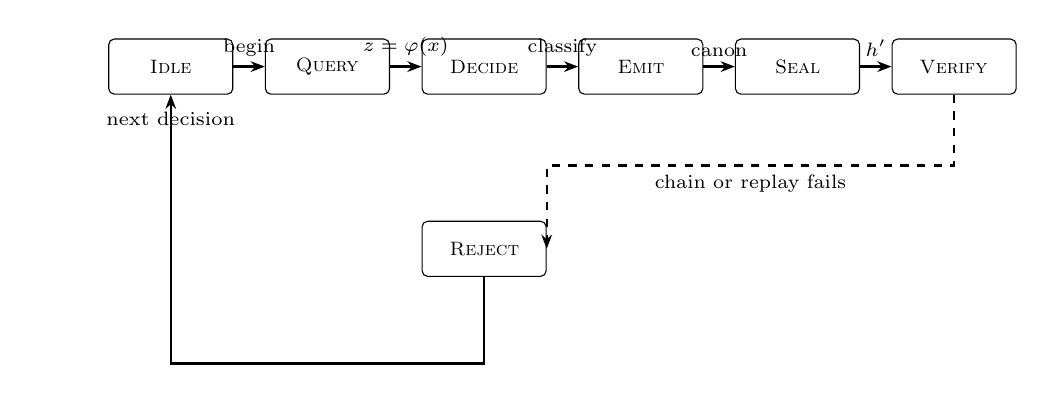
\begin{tikzpicture}[font=\scriptsize, node distance=5mm and 4mm,
  st/.style={draw, rounded corners=2pt, align=center, inner sep=2.5pt, minimum height=7mm, text width=14mm},
  tr/.style={-{Stealth[length=1.8mm]}, thick},
  rej/.style={-{Stealth[length=1.8mm]}, thick, dashed}]
\node[st] (idle) {\textsc{Idle}};
\node[st, right=of idle] (query) {\textsc{Query}};
\node[st, right=of query] (decide) {\textsc{Decide}};
\node[st, right=of decide] (emit) {\textsc{Emit}};
\node[st, right=of emit] (seal) {\textsc{Seal}};
\node[st, right=of seal] (verify) {\textsc{Verify}};
\node[st, below=16mm of decide] (reject) {\textsc{Reject}};
\draw[tr] (idle) -- node[above,font=\scriptsize]{begin} (query);
\draw[tr] (query) -- node[above,font=\scriptsize]{$z=\varphi(x)$} (decide);
\draw[tr] (decide) -- node[above,font=\scriptsize]{classify} (emit);
\draw[tr] (emit) -- node[above,font=\scriptsize]{canon} (seal);
\draw[tr] (seal) -- node[above,font=\scriptsize]{$h'$} (verify);
\coordinate (vdown) at ([yshift=-9mm]verify.south);
\coordinate (rdown) at ([yshift=-11mm]reject.south);
\draw[rej] (verify.south) -- (vdown) -| (reject.east);
\node[font=\scriptsize, anchor=south] at ([yshift=0.6mm]$(reject.east)!0.5!(vdown)$) {chain or replay fails};
\draw[tr] (reject.south) -- (rdown) -| (idle.south);
\node[below=1mm of idle, font=\scriptsize, text width=34mm, align=center] {next decision};
\end{tikzpicture}
\caption{Decision protocol. A decision is classified, emitted as a canonical record, sealed into the hash chain, and verified. Verification failure is terminal for the run: it invalidates the whole record set, not the single record, because a broken chain makes every later digest untrustworthy. Blind spots and conflicts are decision classes, not errors, and they do not trigger the reject edge.}
\label{fig:fsm}
\end{figure}

\subsection{Matched-support symbol intervention}
\label{sec:method-interv}

To test whether a learned symbol causally affects a receiver, we manipulate it while holding everything else fixed. Let $u$ denote the token at the position of interest, $y$ the remaining tokens, and $P_{B}(C\mid u,y)$ the receiver's probability of the target action. The effect is
\begin{equation}
\label{eq:interv}
\Delta_{\iota}(u',u'') \;=\; \mathbb{E}_{\,y\sim\widehat{P}(y)}\Bigl[\, P_{B}(C\mid u',y) - P_{B}(C\mid u'',y) \,\Bigr],
\end{equation}
where the expectation is taken over contexts on which both token values have support. Support matching uses the minimum-mass overlap of Eq.~\eqref{eq:overlap},
\begin{equation}
\label{eq:overlap}
\omega(u',u'') \;=\; \sum_{y} \min\bigl(\widehat{P}(y\mid u'), \widehat{P}(y\mid u'')\bigr),
\end{equation}
and contexts are reweighted so that the two conditional distributions agree. \emph{Protocol-join check.} Eq.~\eqref{eq:interv} compares two conditional distributions of the \emph{same} receiver under the \emph{same} continuation; it therefore estimates an intervention effect on a decision, not the semantic content of the symbol. A large $\Delta_{\iota}$ is compatible with a symbol whose meaning is uninterpretable to a human reader.

\subsection{Diagnostic-only comparator}
\label{sec:method-gpi}

Fitted-Q value estimates with generalised policy improvement \citep{barreto2017,thakoor2022} are included as a \emph{diagnostic}. They are not part of the primary claim, and they carry a pre-declared quality gate: a value-based comparator is admissible only if its greedy action agrees with a reference action source at a rate we fixed before running it, and if its own value direction is identifiable. Section~\ref{sec:res-gpi} reports that the gate fails; the comparator's policy scores are therefore reported as non-claims.

\subsection{Statistical conventions}
\label{sec:method-stats}

\paragraph{Paired estimand.} For two policies evaluated on the same $n$ reset seeds with per-episode returns $G_{i}(\cdot)$, the estimand is the paired mean difference of Eq.~\eqref{eq:estimand},
\begin{equation}
\label{eq:estimand}
\Delta(\pi_{f},\pi_{b}) \;=\; \frac{1}{n}\sum_{i=1}^{n}\bigl(G_{i}(\pi_{f}) - G_{i}(\pi_{b})\bigr),
\end{equation}
with a percentile bootstrap interval over episodes \citep{agarwal2021}. Pairing on reset seed is what makes the comparison interpretable at all, since episode return has very high variance across seeds.

\paragraph{Behavioural agreement.} Agreement is reported in two forms. The pooled estimate is a simple fraction of states. The episode-cluster balanced estimate of Eq.~\eqref{eq:agree} weights each source episode equally,
\begin{equation}
\label{eq:agree}
\bar{A}_{s,s'} \;=\; \frac{1}{m}\sum_{e=1}^{m}\frac{1}{|S_{e}|}\sum_{x\in S_{e}} \mathbf{1}\bigl[\pi_{s}(x)=\pi_{s'}(x)\bigr],
\end{equation}
where $S_{e}$ is the set of sampled states drawn from episode $e$'s occupancy and $m$ the number of episodes. Equation~\eqref{eq:agree} is the estimator we treat as primary, because a pooled fraction would over-weight episodes that contribute more sampled states.

\paragraph{Dispersion.} Where a standard deviation is reported, it is the sample standard deviation across the $100$ evaluation episodes within one policy and one condition. It is never a cross-seed or cross-run quantity unless stated.

\paragraph{Deterministic quantities.} Hash-chain validity, replay equality and codec round-trip are deterministic checks. Their variance is structurally zero: a single failure invalidates the run, and a pass is a property of the recorded bytes rather than a statistical estimate. We report them as counts and never as effects.

\paragraph{Language.} We avoid the word \emph{significant} for the paired differences because no hypothesis test was preregistered for them; we report point estimates and intervals and let the intervals speak.

% =====================================================================
\section{Experimental Setup}
\label{sec:setup}

\subsection{Tasks, agents and arms}

Two control tasks from the standard interface \citep{towers2024} are used: CartPole-v1 ($d=4$, $|\mathcal{A}|=2$, $500$-step cap) and Acrobot-v1 ($d=6$, $|\mathcal{A}|=3$, $500$-step cap). Source policies are single-hidden-layer actors trained with REINFORCE \citep{williams1992} for $300$ episodes per seed and arm, with eight seeds per task. Three arms are trained: an unconstrained baseline, an audit-only observer that records but does not constrain, and a rule-constrained arm. Baseline and audit-only arms are checked for training equivalence by comparing actor-weight and transition-trace digests; every pair matched in every run we report.

The symbolizer is fitted from $24$ random-policy calibration episodes per seed, pooled within the environment, with $b=4$ bins per dimension, and frozen before any scored training (Eq.~\eqref{eq:sym}).

\subsection{Admission, evaluation and controls}

Rules are admitted at $s_{\min}=8$ with $c_{\min}=0.70$ unless stated; a $c_{\min}=0.90$ condition is reported where relevant. Primary policy evaluation uses $100$ identical reset seeds per policy, so all policies in a comparison see exactly the same episode initialisations. The fallback actor is selected from training-return metadata only.

Arbiter ablations re-evaluate the same $100$ reset seeds under nine alternative selection rules. Random selection among available source rules is repeated with five independent selector streams, and a separate control draws one of the three environment actions uniformly and independently at each step with five independent policy streams. The uniform-action control exists to separate \emph{state-conditioned} rule selection from \emph{unconditioned} action noise.

\subsection{Behavioural agreement experiment}

Two frozen CartPole actors (seeds 11 and 29) are applied to the same $10{,}000$ fresh raw states. States are collected from new deterministic rollouts on reset ranges disjoint from all training and evaluation ranges: $100$ episodes for seed 11 and $100$ for seed 29, yielding $50{,}000$ and $13{,}085$ candidate states respectively. We sample $5{,}000$ states without replacement from each actor's own occupancy, so each occupancy contributes equally, and evaluate both actors on the union. Intervals are episode-cluster bootstrap intervals. Training-trace states are never used as held-out observations.

\subsection{Designed symbol task}

The symbol-intervention study uses a separate designed task in which a sender observes one of ten private labels and a receiver must select a parity-dependent target action, with no other channel available: the receiver's image and label inputs are held constant. Symbols are categorical indices over a frozen quantized latent dictionary of size $32$, emitted as sequences of length $2$ \citep{vandenoord2017,liu2025aim}. Each run performs $100{,}000$ episodes in batches of $8$, giving $12{,}500$ optimizer updates. Six seeds are analysed, one extended run plus five independent replications, giving $600{,}000$ logged decisions. The information-bearing token position is selected by held-out mutual information and is seed-dependent; both positions' diagnostics are retained.

\subsection{Unit of analysis and exclusions}

The unit of analysis is the evaluation episode for return estimands, and the state for agreement estimands. Rule statistics are computed per seed. No episode or seed is excluded from any reported aggregate. Two configuration asymmetries are disclosed rather than corrected: the CartPole validation pool retained $39{,}173$ rows against $40{,}000$ for Acrobot because one seed contributed fewer validation candidates than the cap, and the earlier pilot used independently fitted per-seed symbolizers, so we report those numbers as historical and never pool them with the shared-symbolizer results.

\subsection{Registered predictions}
\label{sec:setup-pred}

Table~\ref{tab:pred} lists the predictions we fixed before analysing the shared-symbolizer runs. No external preregistration record exists, so we label them \emph{unregistered} and treat them as post-hoc for the purposes of claim strength.

\begin{table}[H]
\centering
\caption{Predictions fixed before the shared-symbolizer analysis. All are unregistered: no external preregistration record exists, so they are treated as post hoc when assessing claim strength. Each receives a status in Section~\ref{sec:results}.}
\label{tab:pred}
\small
\begin{tabularx}{\textwidth}{@{}l X l@{}}
\toprule
\textbf{ID} & \textbf{Prediction} & \textbf{Budget} \\
\midrule
P1 & Hash-chain, ledger and replay checks pass on all recorded runs under the audited configuration. & CB6 \\
P2 & The lossless codec reconstructs every trace prefix exactly. & CB6 \\
P3 & Baseline and audit-only arms are training-equivalent. & CB6 \\
P4 & Cross-seed rule overlap is substantially above zero under a shared symbolizer. & CB1 \\
P5 & Two actors with high rule overlap also agree on most fresh held-out states. & CB2 \\
P6 & Fused mean return exceeds the best single source actor on both tasks. & CB3 \\
P7 & Blind spots, not conflicts, are the main obstacle to fusion. & CB3 \\
P8 & The deployed confidence-ranked arbiter is at least as good as the alternative selection rules. & CB4 \\
\bottomrule
\end{tabularx}
\end{table}

\subsection{Ethics}

No human participants, annotators, or human-subject data are involved in this study. All experiments are computational, use synthetic or standard benchmark environments, and involve no personal data, consent, compensation, withdrawal, or institutional approval. We state this explicitly rather than by omission: the absence of an ethics section would be ambiguous, whereas the absence of human subjects is a fact about the design.

% =====================================================================
\section{Results}
\label{sec:results}

\subsection{Trace integrity, ledger and replay}
\label{sec:res-audit}

\textbf{P1 and P2 --- supported.} Across the eight-seed runs, audit records cover $1{,}725{,}655$ CartPole rows and $2{,}544{,}513$ Acrobot rows; environment replay checks cover $1{,}122{,}403$ and $1{,}742{,}570$ transitions respectively. Every hash-chain check passed and every replayed transition matched exactly on state, next state, reward, termination and truncation. Optimizer-update ledgers contain $7{,}200$ records per task. Rule-provenance snapshots resolved $290{,}052$ CartPole and $697{,}817$ Acrobot decision references back to source rules.

Cold reruns of two seeds reproduced actor weights, transition traces, all $300$ per-episode update records and the final checkpoint; across those two seeds $135{,}427$ distinct transition records were each compared twice, giving $270{,}854$ exact comparisons. Table~\ref{tab:audit} summarises.

\begin{table}[H]
\centering
\caption{Audit and replay coverage for the eight-seed runs. These are deterministic checks: the variance is structurally zero, a pass is a property of the recorded bytes, and a single failure would invalidate the run rather than reduce a rate. Reported as counts, not as effects.}
\label{tab:audit}
\small
\begin{tabular}{@{}lrr@{}}
\toprule
\textbf{Quantity} & \textbf{CartPole-v1} & \textbf{Acrobot-v1} \\
\midrule
Recorded trace rows (all arms) & $1{,}725{,}655$ & $2{,}544{,}513$ \\
Optimizer-update records & $7{,}200$ & $7{,}200$ \\
Replayed environment transitions & $1{,}122{,}403$ & $1{,}742{,}570$ \\
Decision references resolved to rules & $290{,}052$ & $697{,}817$ \\
Chain-validation failures & $0$ & $0$ \\
Replay mismatches & $0$ & $0$ \\
\bottomrule
\end{tabular}
\end{table}

\subsection{Lossless coding and its limits}

\textbf{P2 --- supported.} For CartPole the trace contains $9{,}178{,}724$ lexical tokens reduced to a $16$-production grammar, and for Acrobot $8{,}549{,}496$ tokens. Every trace prefix round-tripped exactly with matching digests. The byte comparison is the interesting part, and it is unflattering: the grammar archive is $13{,}377{,}210$ bytes against $61{,}295{,}430$ bytes for the raw trace ($78.2\%$ smaller), but $12{,}341{,}225$ bytes of ordinary compression achieves more, leaving the grammar archive $8.4\%$ \emph{larger} than plain compression. Acrobot shows the same pattern ($13{,}738{,}167$ against $12{,}499{,}612$ bytes, $9.9\%$ larger). The two-part code length falls monotonically in absolute terms but its ratio to the raw encoding does not improve after the first round ($0.513, 0.536, 0.549, 0.561, 0.575, 0.575$ across six $50$-episode rounds), and at $300$ episodes it reaches $281{,}958{,}036$ bits against $490{,}363{,}440$ raw UTF-8 bits.

We draw a narrow conclusion. The codec preserves structure and reconstructs exactly; it is not a competitive compressor, and its induction procedure does not optimise the code length it is being scored by. Reporting the code length as a proxy for rule quality would be a category error.

\subsection{Rule overlap across seeds}
\label{sec:res-overlap}

\textbf{P4 --- supported.} Under the shared symbolizer, mean pairwise rule Jaccard across the eight CartPole seeds is $0.5572$ (median $0.5725$) and across the eight Acrobot seeds $0.0956$ (median $0.0590$). The seed 11/29 pair reaches $0.5833$ on CartPole with $77$ shared and $132$ union productions, and $0.0496$ on Acrobot with $21$ shared and $423$ union.

\begin{table}[H]
\centering
\caption{Rule overlap and its internal consistency. The contrast between tasks is the first sign that a high overlap number can be a property of the task rather than of the agents' agreement. Acrobot's all-seed intersection is empty of agreement: both shared conditions conflict.}
\label{tab:overlap}
\small
\begin{tabular}{@{}lcc@{}}
\toprule
\textbf{Quantity} & \textbf{CartPole-v1} & \textbf{Acrobot-v1} \\
\midrule
Mean pairwise Jaccard (8 seeds) & $0.5572$ & $0.0956$ \\
Median pairwise Jaccard & $0.5725$ & $0.0590$ \\
Seed 11/29 Jaccard & $0.5833$ & $0.0496$ \\
Seed 11/29 shared productions & $77$ & $21$ \\
Seed 11/29 union of productions & $132$ & $423$ \\
Shared conditions with conflicting actions (11/29) & $0$ of $77$ & $77$ of $98$ \\
All-seed intersection / same-action core & $38$ / $38$ & $2$ / $0$ \\
\bottomrule
\end{tabular}
\end{table}

Table~\ref{tab:overlap} also exposes the first counterexample. On Acrobot, the intersection of all eight seeds' rule banks contains two conditions and \emph{both} conflict: the only symbolic states that all eight agents agree are worth encoding are states on which they disagree about the action. A single aggregate ``shared core size'' would report $2$ and hide this entirely.

\subsection{Behavioural agreement: overlap is not consensus}
\label{sec:res-agree}

\textbf{P5 --- contradicted.} Applying the two frozen CartPole actors to the same $10{,}000$ fresh raw states gives $5{,}138$ agreements, a pooled rate of $51.38\%$. The episode-cluster balanced estimate is $51.36\%$ with a 95\% bootstrap interval of $[50.48, 52.26]$. Per-occupancy rates are $50.56\%$ (seed 11 occupancy) and $52.20\%$ (seed 29 occupancy). Stratifying by absolute pole angle gives $50.16\%$ near zero ($n=7{,}807$), $55.77\%$ in a middle band ($n=2{,}182$), and $45.45\%$ in a large-angle band with only $n=11$, too few to interpret.

For a two-action task, $51.36\%$ is essentially chance. The two agents whose rule sets overlap by $0.5833$ do not share a policy core in any behavioural sense we can measure. Figure~\ref{fig:overlap-agree} places the two quantities side by side; the visual point is that the height of the left bar carries no information about the height of the right one.

\begin{figure}[t]
\centering
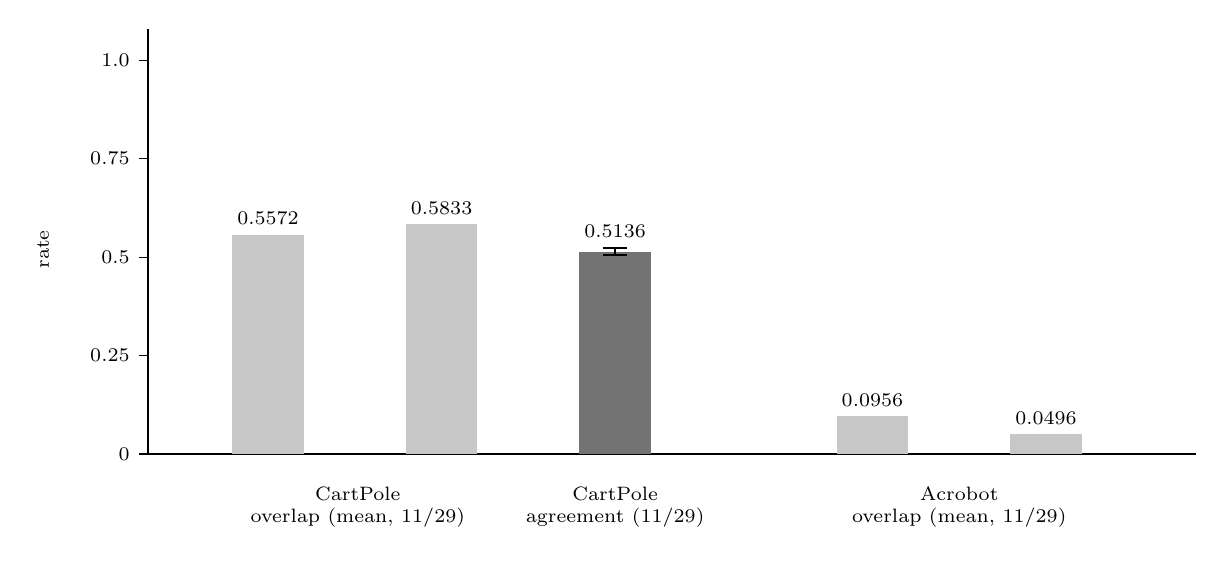
\begin{tikzpicture}[font=\footnotesize, x=38mm, y=50mm]
% axes
\draw[thick] (0,0) -- (0,1.08);
\draw[thick] (0,0) -- (3.5,0);
\foreach \v in {0,0.25,0.5,0.75,1.0} {%
  \draw (0,\v) -- (-0.03,\v) node[left,font=\scriptsize]{\v};}
\node[rotate=90, anchor=south, font=\scriptsize] at (-0.30,0.52) {rate};
% bars
\fill[black!22] (0.28,0) rectangle (0.52,0.5572);
\fill[black!22] (0.86,0) rectangle (1.10,0.5833);
\fill[black!55] (1.44,0) rectangle (1.68,0.5136);
\fill[black!22] (2.30,0) rectangle (2.54,0.0956);
\fill[black!22] (2.88,0) rectangle (3.12,0.0496);
% CI whisker on the behavioural bar
\draw[thick] (1.56,0.5048) -- (1.56,0.5226);
\draw[thick] (1.52,0.5048) -- (1.60,0.5048);
\draw[thick] (1.52,0.5226) -- (1.60,0.5226);
% value labels
\node[above,font=\scriptsize] at (0.40,0.5572) {0.5572};
\node[above,font=\scriptsize] at (0.98,0.5833) {0.5833};
\node[above,font=\scriptsize] at (1.56,0.5260) {0.5136};
\node[above,font=\scriptsize] at (2.42,0.0956) {0.0956};
\node[above,font=\scriptsize] at (3.00,0.0496) {0.0496};
% group labels
\node[below,font=\scriptsize,align=center] at (0.70,-0.06) {CartPole\\overlap (mean, 11/29)};
\node[below,font=\scriptsize,align=center] at (1.56,-0.06) {CartPole\\agreement (11/29)};
\node[below,font=\scriptsize,align=center] at (2.71,-0.06) {Acrobot\\overlap (mean, 11/29)};
\end{tikzpicture}
\caption{Rule overlap and behavioural agreement are different quantities. Darker bars are behavioural measurements; lighter bars are set statistics. The whisker on the middle bar is the 95\% episode-cluster bootstrap interval $[50.48,52.26]$, which contains the $50\%$ chance level for a two-action task. Overlap of $0.5833$ coexists with agreement indistinguishable from chance. Note that the Acrobot overlap bars are low not because the agents agree but because they encode almost disjoint symbolic conditions (Table~\ref{tab:overlap}).}
\label{fig:overlap-agree}
\end{figure}

\subsection{Composition returns and the decision mix}
\label{sec:res-returns}

\textbf{P6 --- partially supported.} Table~\ref{tab:returns} gives held-out returns. On CartPole the fused policy reaches $205.96$ against $163.65$ for the best single actor (paired difference $+42.31$, 95\% interval $[23.98, 61.93]$), but the actor-logit ensemble reaches $500.00$, the environment's step cap. CartPole's return scale is therefore saturated for some policies and the fused-versus-best comparison is compressed by the ceiling.

On Acrobot the fused policy reaches $-443.37$ against $-500.00$ for both the best single actor and the ensemble (paired difference $+56.63$, interval $[39.32, 75.15]$). The mean must be read with the median: the median is $-500.00$, and $39$ of $100$ episodes terminate above $-500$. The difference is therefore carried by a minority of episodes that reach the goal early, not by a uniform improvement.

\begin{table}[H]
\centering
\caption{Held-out returns over $100$ identical reset seeds per task, with paired differences against the best single source actor and percentile bootstrap intervals over episodes. The Acrobot standard deviation of $0.00$ for the ensemble is structural: every episode hits the return floor, which is a property of the task and the policy, not evidence of stability. CartPole's $500.00$ is the environment's step cap.}
\label{tab:returns}
\small
\begin{tabular}{@{}lrrrr@{}}
\toprule
\textbf{Policy} & \textbf{Mean} & \textbf{Median} & \textbf{SD} & \textbf{Paired $\Delta$ vs best single [95\%]} \\
\midrule
CartPole best single actor & $163.65$ & $137.0$ & $50.35$ & --- \\
CartPole actor-logit ensemble & $500.00$ & $500.0$ & $0.00$ & $+336.35\ [326.13,346.21]$ \\
CartPole grammar fusion & $205.96$ & $181.0$ & $79.12$ & $+42.31\ [23.98,61.93]$ \\
\midrule
Acrobot best single actor & $-500.00$ & $-500.0$ & $0.00$ & --- \\
Acrobot actor-logit ensemble & $-500.00$ & $-500.0$ & $0.00$ & $0.00\ [0.00,0.00]$ \\
Acrobot grammar fusion & $-443.37$ & $-500.0$ & $90.77$ & $+56.63\ [39.32,75.15]$ \\
\bottomrule
\end{tabular}
\end{table}

\textbf{P7 --- contradicted, and informatively so.} The decision mix is in Table~\ref{tab:mix}. CartPole is $98.27\%$ covered with $0.36\%$ conflicts and $1.73\%$ blind spots. Acrobot is $95.70\%$ covered, $4.30\%$ blind spots, and $89.24\%$ \emph{conflicts}. The predicted obstacle, blind spots, accounts for $4.30\%$ of decisions, whereas conflicts account for $89.24\%$. The prediction was wrong in the direction that matters: the difficulty is not missing knowledge but incompatible knowledge, and the arbitration rule rather than the rule bank becomes the object of study.

\begin{table}[H]
\centering
\caption{Decision mix under grammar fusion. Coverage and blind-spot rate sum to $1$ by construction; the conflict rate is a subset of coverage. Acrobot's profile --- high coverage, high conflict --- is the opposite of what we predicted and is what motivates the ablation in Section~\ref{sec:res-arb}.}
\label{tab:mix}
\small
\begin{tabular}{@{}lrrr@{}}
\toprule
\textbf{Task} & \textbf{Coverage $\gamma$} & \textbf{Conflict rate $\chi$} & \textbf{Blind-spot rate $\beta$} \\
\midrule
CartPole-v1 & $98.27\%$ ($20{,}240$/$20{,}596$) & $0.36\%$ ($75$) & $1.73\%$ ($356$) \\
Acrobot-v1 & $95.70\%$ ($42{,}467$/$44{,}376$) & $89.24\%$ ($39{,}602$) & $4.30\%$ ($1{,}909$) \\
\bottomrule
\end{tabular}
\end{table}

\subsection{Arbitration sensitivity and the random-selection anomaly}
\label{sec:res-arb}

\textbf{P8 --- contradicted.} Table~\ref{tab:arb} reports nine matched-seed arbiter variants on the same $100$ reset seeds. The deployed confidence-ranked arbiter scores $-443.37$. Confidence-only scores $-444.49$ (paired difference $-1.12$, interval $[-3.16, 0.06]$), which is effectively the same policy. Mean-reward-only, support-first, unanimous-only, deferring conflicts to the actor ensemble, and preferring either single source seed all score exactly $-500.00$. Falling back to the best single actor only on blind spots scores $-452.69$.

Random selection among the available source rules scores $-187.02$ on one selector stream, with a paired difference of $+256.35$ against the deployed arbiter (interval $[231.38, 278.21]$). Five further independent selector streams score $-194.10$, $-195.38$, $-201.46$, $-196.97$ and $-206.17$, a mean of $-198.82$, with paired differences of $+249.27$, $+247.99$, $+241.91$, $+246.40$ and $+237.20$; every interval lies wholly above zero, with lower bounds between $+215.11$ and $+226.90$.

The uniform-random-action control on the same reset seeds averages $-498.71$ over five streams ($-499.98$, $-496.39$, $-497.76$, $-499.85$, $-499.55$). Unconditioned action noise therefore does not reproduce the effect. Because rule availability depends on the symbolic state, a stochastic selector over available rules induces a state-conditioned mixture of source rules, which is a different object from a uniform action policy.

One incidental observation deserves recording because it constrains interpretation. The random-selection runs terminate episodes far earlier: they log roughly $19{,}000$ to $20{,}700$ steps against $44{,}376$ for the deployed arbiter, because episodes end when the task goal is reached. The mean difference is thus partly a statement about episode length under a policy that reaches the goal more often.

We report this as an anomaly with no accepted explanation. It does not show that random arbitration is generally preferable, it does not transfer to any other task as far as we know, and it does not show that the deployed arbiter is badly designed in a way we understand. It does show that our confidence-ranked arbiter is not established as a good conflict resolver, which is a claim we would otherwise have made.

\begin{table}[H]
\centering
\caption{Arbiter ablations on Acrobot-v1, all evaluated on the same $100$ reset seeds. Differences are paired against the deployed confidence-ranked arbiter. The deployed rule is not the best rule tested, and the best rule tested is random selection. The final row is a control, not a policy we propose.}
\label{tab:arb}
\footnotesize
\begin{tabular}{@{}lrrr@{}}
\toprule
\textbf{Selection rule} & \textbf{Mean return} & \textbf{Paired $\Delta$ [95\%]} & \textbf{Steps} \\
\midrule
Deployed confidence-ranked & $-443.37$ & $0.00\ [0.00,0.00]$ & $44{,}376$ \\
Confidence only & $-444.49$ & $-1.12\ [-3.16,0.06]$ & $44{,}488$ \\
Best-single fallback & $-452.69$ & $-9.32\ [-19.51,0.50]$ & $45{,}305$ \\
Prefer source seed 11 & $-499.48$ & $-56.11\ [-74.23,-39.12]$ & $49{,}949$ \\
Prefer source seed 29 & $-500.00$ & $-56.63\ [-74.95,-39.85]$ & $50{,}000$ \\
Mean-reward only & $-500.00$ & $-56.63\ [-75.47,-39.67]$ & $50{,}000$ \\
Support first & $-500.00$ & $-56.63\ [-74.84,-39.68]$ & $50{,}000$ \\
Unanimous only & $-500.00$ & $-56.63\ [-74.49,-39.36]$ & $50{,}000$ \\
Defer conflicts to ensemble & $-500.00$ & $-56.63\ [-75.12,-40.08]$ & $50{,}000$ \\
\midrule
Random rule among available & $-187.02$ & $+256.35\ [231.38,278.21]$ & $18{,}802$ \\
\quad five further streams (mean) & $-198.82$ & $+245.55\ [215.11,226.90]$ & $19{,}801$ \\
\midrule
Uniform random action (control) & $-498.71$ & --- & --- \\
\bottomrule
\end{tabular}
\end{table}

\begin{figure}[t]
\centering
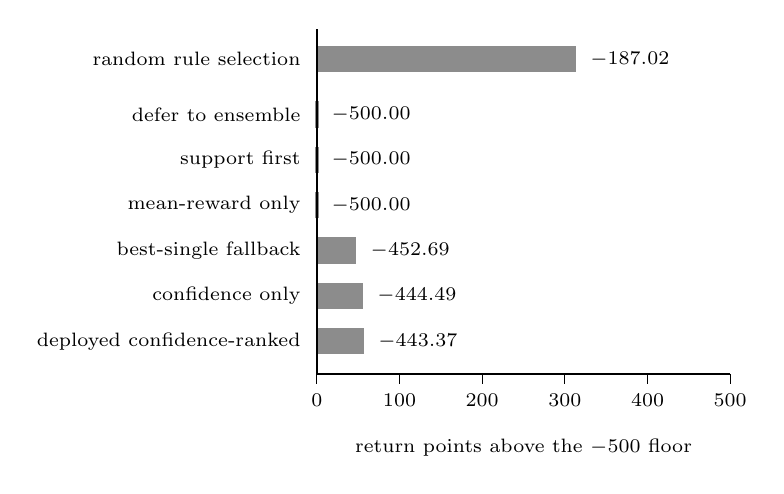
\begin{tikzpicture}[font=\footnotesize, x=0.105mm, y=6.4mm]
% x = 0 is the -500 return floor; one coordinate unit is one return point.
\foreach \r/\lbl/\y in {-443.37/{deployed confidence-ranked}/1.0,
                          -444.49/{confidence only}/1.9,
                          -452.69/{best-single fallback}/2.8,
                          -500.00/{mean-reward only}/3.7,
                          -500.00/{support first}/4.6,
                          -500.00/{defer to ensemble}/5.5,
                          -187.02/{random rule selection}/6.6}{%
  \pgfmathsetmacro{\len}{\r+500}%
  \node[left, font=\scriptsize, anchor=east] at (-8,\y) {\lbl};%
  \ifdim\len pt>1pt
    \fill[black!45] (0,\y-0.26) rectangle (\len,\y+0.26);
    \node[right, font=\scriptsize, anchor=west] at (\len+6,\y) {$\r$};%
  \else
    \draw[black!45,line width=1.2pt] (0,\y-0.26) -- (0,\y+0.26);
    \node[right, font=\scriptsize, anchor=west] at (6,\y) {$\r$};%
  \fi}
\draw[thick] (0,0.35) -- (0,7.2);
\draw (0,0.35) -- (500,0.35);
\foreach \p in {0,100,200,300,400,500}{%
  \draw (\p,0.35) -- (\p,0.15) node[below,font=\scriptsize]{$\p$};}
\node[below,font=\scriptsize] at (250,-0.75) {return points above the $-500$ floor};
\end{tikzpicture}
\caption{Arbiter ablations on Acrobot-v1, drawn from the $-500$ return floor. The four deterministic variants that score exactly $-500.00$ are drawn as ticks at the origin. The deployed confidence-ranked arbiter and the confidence-only variant are indistinguishable; random selection among available source rules is far to the right. The comparison is not a controlled ablation in the causal sense: the variants differ in which decisions they alter, and the random variant also changes episode lengths (Table~\ref{tab:arb}), so this figure shows sensitivity, not an isolated effect of the selection rule.}
\label{fig:arb}
\end{figure}

\subsection{Causal symbol intervention in the designed task}
\label{sec:res-interv}

\textbf{Supported within the designed task.} Across six seeds and $600{,}000$ logged decisions, sender-sampled receiver accuracy averages $0.998923$ (per-seed range $0.997881$ to $0.999827$), against $0.503292$ for shuffled messages and $0.500$ for the no-message control. The matched-support intervention of Eq.~\eqref{eq:interv} on the information-bearing position changes receiver action probability by $0.998366$ on average, per-seed range $0.996986$ to $0.999685$, with mean common-support overlap $0.94308$ (range $0.90852$ to $0.97283$). The active position is seed-dependent: it is position $1$ for four of the six seeds and position $0$ for two.

Two earlier configurations of the same task are instructive and are reported as negative results. With $79$ optimizer updates the receiver showed no channel at all: argmax accuracy $0.500$, matched-support difference $0.00088$ with interval $[-0.00136, 0.00320]$, and position mutual information indistinguishable from permutation null. The cause was identified: batching had reduced the number of optimizer steps by roughly two orders of magnitude relative to the single-step design. With $1{,}250$ updates the effect appeared but was partial, with argmax accuracy $0.800$ against sampled accuracy $0.6008$ --- a gap that would have been hidden by an argmax-only report. Full strength required the complete $12{,}500$ updates.

The scope of this result is narrow by construction. Equation~\eqref{eq:interv} shows that the symbol at one position changes a decision in this task. It does not show that the symbol sequence is human-readable, that other positions carry meaning, or that the same mechanism operates in the control tasks, where the symbolic objects are induced state--action rules rather than learned message tokens.

\subsection{The value-based comparator fails its own gate}
\label{sec:res-gpi}

\textbf{Non-claim.} The pre-declared admissibility gate fails on both tasks. On CartPole the fitted-Q greedy action agrees with the actor-logit ensemble on $35.27\%$ of $31{,}563$ held-out states, and the comparator's own evaluation return is $9.34$ against $163.65$ for the best actor (paired difference $-154.31$, interval $[-164.38,-144.65]$). On Acrobot it scores $-499.57$ and selects action $0$ on all $50{,}000$ diagnostic states, with $0.00\%$ agreement with the ensemble.

The failure is more informative than the score. On a $200$-state Acrobot sample, the two seeds' Q vectors correlate at $0.652$, yet their greedy actions diverge almost completely: seed 11 selects action $1$ on $186$ of $200$ states while seed 29 selects action $0$ on all $200$. Scalar value correlation is therefore not action-value agreement. Comparing the fused action against several references gives $64.5\%$ agreement with the seed-11 critic's argmax (interval $[58.0,71.0]$), $0\%$ with seed 29's, $0\%$ with multi-critic generalised policy improvement, and $22.5\%$ with the best first action under a fixed actor-ensemble continuation (interval $[16.5,28.5]$); mean regret against that continuation is $108.24$ return points (interval $[86.10,132.03]$). The last quantity estimates action values for the stated continuation policy, not for an optimal policy.

We report these as diagnostics only. They are the reason the paper contains no comparison against value-based composition: we could not construct a value-based comparator that passed its own quality gate, and reporting its policy scores as a result would be reporting a defect as a finding.

\subsection{Summary of verdicts}

Table~\ref{tab:verdicts} separates outcomes by the layer of evidence they belong to. The distinction matters because several of the most emphatic results in this paper --- every chain check passing, every transition reproducing --- carry no identification weight at all: they are deterministic checks that a correct implementation passes by construction.

\begin{table}[H]
\centering
\caption{Outcome summary. The \emph{layer} column separates identification-bearing results from deterministic and diagnostic ones. A deterministic check that passes is not evidence for a scientific claim; a deterministic check that failed would have been evidence of a defect.}
\label{tab:verdicts}
\small
\begin{tabular}{@{}p{52mm} r r >{\raggedright\arraybackslash}p{36mm}@{}}
\toprule
\textbf{Criterion} & \textbf{Estimate} & \textbf{Threshold} & \textbf{Verdict / layer} \\
\midrule
Chain integrity, replay equality & $0$ failures & $0$ & pass --- operational health \\
Codec round-trip on all prefixes & exact & exact & pass --- diagnostic \\
Baseline/audit training equivalence & digests equal, $8/8$ & equality & pass --- design integrity \\
CartPole mean pairwise rule overlap & $0.5572$ & $>0$ & pass --- identification (CB1) \\
CartPole 11/29 behavioural agreement & $51.36\%$ & $\gg 50\%$ & \textbf{fail} --- identification (CB2) \\
CartPole fused vs best single & $+42.31$ & $>0$ & pass, ceiling-limited (CB3) \\
Acrobot fused vs best single & $+56.63$ & $>0$ & pass, median unchanged (CB3) \\
Blind spots as the main obstacle & $4.30\%$ & dominant & \textbf{fail} --- conflicts dominate (CB3) \\
Deployed arbiter is competitive & $-443.37$ & best of set & \textbf{fail} --- random scores $-187.02$ (CB4) \\
Symbol intervention effect & $0.998366$ & $\gg 0$ & pass --- identification (CB5) \\
Value comparator admissible & $35.27\%$, $0.00\%$ & pre-declared gate & \textbf{fail} --- non-claim \\
\bottomrule
\end{tabular}
\end{table}

% =====================================================================
\section{Discussion}
\label{sec:discussion}

\subsection{Why the surviving mechanism may work}

The parts of the system that behave as intended share a property: they are deterministic transformations with an explicit input and output space, joined to the next stage by a checkable predicate. The symbolizer is a fixed quantile map (Eq.~\eqref{eq:sym}). Admission is a threshold on two well-defined statistics (Eq.~\eqref{eq:admit}), and Proposition~\ref{prop:partial} guarantees the resulting bank is a partial function, which is what makes the decision partition of Eq.~\eqref{eq:partition} exhaustive and disjoint. The chain (Eq.~\eqref{eq:chain}) and the replay predicate (Eq.~\eqref{eq:replay}) are equality tests over canonical bytes.

The parts that behave poorly are exactly the parts where a \emph{choice} has to be made without evidence: which candidate action to prefer at a conflict. Equation~\eqref{eq:arb} encodes a reasonable-sounding preference order, and Section~\ref{sec:res-arb} shows the order is not supported. We read the contrast as the central methodological lesson of the study: audit mechanisms that are reductions can be made correct and verifiable, whereas arbitration policies are empirical objects that must be measured, and our measurements did not confirm the one we built.

\subsection{Prediction outcomes}

Of the eight predictions, three were supported (P1, P2, P4), two were partially supported (P3, P6), and three were contradicted (P5, P7, P8). The contradicted predictions are the informative ones. P5 assumed that symbolic overlap implies behavioural agreement; the measurement puts agreement at chance. P7 assumed blind spots would be the binding constraint; on Acrobot conflicts outnumber blind spots by a factor of twenty. P8 assumed the deployed arbiter was at least as good as alternatives; a random alternative is better by a wide margin. A study that had reported only P1, P2 and P4 would have looked considerably more successful and would have supported none of the conclusions this paper actually draws.

\subsection{Alternative explanations for the unexpected result}

The random-selection advantage admits at least three explanations, and we can rule out none of them.

\emph{Explanation 1: the comparison is not like-for-like.} The random variant logs roughly $19{,}000$ to $20{,}700$ steps against $44{,}376$, because episodes terminate earlier when the goal is reached. A policy that reaches the goal more often produces shorter episodes, and mean return and episode length are entangled here. The correct comparison would hold the decision set fixed, which the current design does not.

\emph{Explanation 2: the deterministic arbiter is systematically biased, not merely noisy.} Confidence and support are computed on the audit-only arm's occupancy. A rule with high confidence on that occupancy may be poorly calibrated on the evaluation occupancy. A random selector avoids this by construction, so its advantage could be a statement about distribution shift rather than about arbitration.

\emph{Explanation 3: the effect is an artefact of the mean-reward degeneracy.} Remark~\ref{rem:degenerate} shows the third arbitration key is constant for $1{,}575$ of $1{,}694$ Acrobot rules. The deterministic variants that rely on that key collapse to a fixed tie order, which may be systematically worse than chance rather than merely uninformative. This would make the finding a statement about a degenerate statistic, not about determinism.

These explanations are not mutually exclusive, and distinguishing them requires the occupancy-stratified decomposition listed as future work.

\subsection{Implications}

\paragraph{Theoretical.} Auditability decomposes. The six questions in Figure~\ref{fig:questions} are not facets of one property but independent predicates, and the evidence here shows they can point in opposite directions: our records are maximally intact while our rule-based account of behaviour is at chance. Any framework that scores auditability as a scalar is therefore measuring the framework's aggregation, not the system's property.

\paragraph{Practical.} Two design consequences follow. First, a rule-fusion layer should publish its decision mix, because the same mean return means different things at $89.24\%$ conflict and at $1.73\%$ conflict. Second, if a system must attribute a decision to a named source, then the arbitration rule must be treated as an empirical component with its own evaluation, not as a preference statement in a specification. We did not do this before building, and the ablation is what told us.

We make no claim about downstream training or deployment effects; no such experiment was run.

\subsection{Steelman}

The strongest objection to this paper is that it reports a negative result about a mechanism it designed, and that the negative result is an artefact of that design rather than a fact about symbolic rule fusion. On this reading, the $51.36\%$ agreement figure is not evidence that symbolic overlap fails to track behaviour, but evidence that \emph{our} symbolizer is too coarse: four quantile bins per dimension fitted to random-policy rollouts is a deliberately weak representation, and two actors whose representations disagree because the representation is weak tells us nothing about rule fusion in general. Similarly, the random-selection advantage may be a property of a degenerate reward statistic rather than a fact about arbitration. This objection is largely correct, and it does not weaken our conclusions, because our conclusions are already restricted to what this configuration shows. What the objection does undermine is any attempt to read the paper as a general negative verdict on rule-level composition, and we do not offer one. What survives is narrower and, we think, still useful: on this configuration, an overlap statistic computed on induced rules carries no information about behavioural agreement, and a plausible preference-based arbiter was not confirmed by its own ablation. Both are falsifiable statements about a specified system, and both were contrary to our expectations before measurement.

\subsection{Replication analysis}

\emph{Likely replication failures.} Three are foreseeable. (i) The arbitration result is sensitive to the selector stream: the initial stream gave $-187.02$ while five later streams ranged to $-206.17$, so a single-stream replication would report a different magnitude. (ii) The Acrobot result depends on the return floor: with a median of $-500.00$, a replication with different reset seeds could shift the mean substantially without changing any qualitative conclusion. (iii) The behavioural agreement result depends on the symbolizer, which is fitted to random-policy occupancy; a replication with a different calibration policy could move it.

\emph{Evidenced mitigations.} Sharing one symbolizer across seeds and arms within a task is \textsc{high} --- it removes the largest known confound in cross-seed comparison and is directly evidenced by the boundary differences of up to $0.1569$ observation units observed under per-seed fitting. Pairing all policy comparisons on identical reset seeds is \textsc{high} --- it is what makes the paired differences interpretable at all given the return variance. Reporting the decision mix alongside every fused return is \textsc{medium} --- it prevents the most likely misreading, though it does not by itself explain the returns. Repeating the random-selection condition across five independent streams is \textsc{medium} --- it establishes that the effect is not a single-stream artefact, but it does not identify the mechanism.

\emph{Replaying a record is not regenerating it.} Our replay results re-execute recorded actions; they do not regenerate a policy. A replication attempt that retrains from scratch is a different experiment from one that replays our traces, and the two should not be compared as if they measured the same thing. For independent replication, the minimum package is: the frozen symbolizer boundaries for each task, the admitted rule banks with their support and confidence statistics, the evaluation reset seed ranges, and the decision traces with their chain digests. The unresolved dependency is the software and hardware configuration, which we cannot guarantee is reproducible elsewhere.

% =====================================================================
\section{Limitations}
\label{sec:limits}

\paragraph{Experimental design.} Two benchmark control tasks, eight seeds each, one shared symbolizer per task, one calibration policy. The symbolizer is fitted to random-policy occupancy and is therefore not optimised for the states the trained policies actually visit. CartPole's return scale is saturated at the step cap for some policies, which compresses the fused-versus-best comparison; Acrobot's median return sits at the floor, so mean comparisons are carried by a minority of episodes.

\paragraph{Reproducibility boundary.} Exact replay is bounded to the recorded software stack and a single CPU host configuration. It cannot establish cross-hardware equivalence, and it does not prove that the recorder captured every cause.

\paragraph{Measurement reliability.} The behavioural agreement experiment measures one pair of actors on one task. It is not a sample of agent pairs, and we do not extend it to the eight-seed mean overlap figures. The episode-cluster balanced estimator was chosen over the pooled fraction because the pooled fraction over-weights high-occupancy episodes, but we report both.

\paragraph{Confounders and negative results.} The arbitration comparison is confounded with episode length, as the random variant reaches the goal more often and logs far fewer steps. The mean-reward arbitration key is degenerate on Acrobot. The value-based comparator failed its pre-declared gate and contributes no comparison. A per-seed symbolizer condition and a rule-constrained training condition were both abandoned after producing unstable results, and those questions are left unanswered rather than answered negatively.

\paragraph{External validity.} Nothing here shows that rule overlap fails to predict behaviour on other tasks, that random arbitration is generally preferable, or that the symbol-intervention result generalises beyond the designed parity task.

\paragraph{Material gap.} The symbolic design underlying the designed task originates from a separate project whose formal reference was not available to us at the time of writing; we therefore cite the symbol-system design at the level of its published description only and make no further claims about it.

% =====================================================================
\section{Conclusion}
\label{sec:conclusion}

We set out to determine what a replayable trajectory plus a set of induced rules can support, and we found that the answer splits cleanly along a line we had not drawn in advance. Deterministic, reduction-like components behaved as specified: every one of $1{,}725{,}655$ CartPole and $2{,}544{,}513$ Acrobot recorded rows passed chain validation, every replayed transition reproduced exactly, and every trace prefix round-tripped losslessly. Empirical, choice-like components did not: two agents whose rule sets overlap by $0.5833$ agreed on $51.36\%$ of actions on fresh states, the obstacle to composition turned out to be conflicts rather than blind spots by a factor of twenty, and the deployed arbitration rule was beaten by random selection among the available rules. A value-based comparator could not be made to pass its own quality gate and is reported as a non-claim.

The claim we are prepared to defend is bounded: in these settings, a provenance-aware rule layer makes the composition of learned rules inspectable, attributable and replayable, and it does so while publishing the decision classes that determine how its returns should be read. Generality, universal causal explanation, and complete auditability of arbitrary reinforcement learning training remain unproven, and the counterexamples in this paper are the reason we do not claim them.

\bibliographystyle{plainnat}
\bibliography{references}

\end{document}
